\section{Theorie}
\label{sec:Theorie}

Für die Vakuumphysik gibt es zahlreiche Anwendungsfelder, wie etwa die 
Lebensmittelindustrie, die chemische oder Halbleiterindustrie. Um Vakuumc, 
also einen Raum mit einem Druck, geringer als dem Druck in der Atmosphäre, zu 
erzeugen und zu charakterisieren, sind spezielle Komponenten, Pumpen und
Messgeräte notwendig, deren Zusammenspiel und physikalische Grundlagen im
Folgenden erläutert werden.

\subsection{Terminologie und Definitionen der Vakuumtechnik}
Neben dem Begriff des Vakuums spielt auch der Rezipient eine elementare Rolle. 
Dieser ist eine Kammer, welche ein Gas in einem Niederdruck beinhaltet (hier:
das Vakuum). Weiter wichtig sind der Totaldruck und der Partialdruck, wobei 
ersteres jener Druck ist, welcher entsteht, wenn die Gasteilchen auf Wände der 
Gaskammer treffen. Der Partialdruck ist der Druck eines spezifischen Gases. Für 
ein Gemisch können die Partialdrücke aufsummiert werden. 
\\
Um Druckbereiche einfacher zu differenzieren wird in die Folgenden unterteilt:
\begin{align*}
    \text{Grobvakuum (GV)}: & \quad \qty{1}{\bar} \text{ bis } \qty{1}{\milli\bar} \quad (\text{Atmosphärendruck}) \\
    \text{Feinvakuum (FV)}: & \quad \qty{1}{\milli\bar} \text{ bis } \qty{e-3}{\milli\bar} \quad (\text{z.B. in der Thermoskanne}) \\
    \text{Hochvakuum (HV)}: & \quad \qty{e-3}{\milli\bar} \text{ bis } \qty{e-7}{\milli\bar} \quad (\text{In Röntgenröhren}) \\
    \text{Ultrahochvakuum (UHV)}: & \quad \qty{e-7}{\milli\bar} \text{ bis } \qty{e-12}{\milli\bar} \quad (\text{In Teilchenbeschleunigern}) \\
    \text{Extremes Ultrahochvakuum (XHV)}: & \quad \text{ weniger als } \qty{e-12}{\milli\bar} \quad (\text{Im Weltraum}) \\
\end{align*}
\noindent Je nach Druckbereich variiert die mittlere freie Weglänge, ein Maß 
für die Distanz, welche ein Teilchen im Mittel zwischen zwei Stößen zurücklegt. 
Diese spielt eine wichte Rolle für die Turbomolekularpumpe (siehe \autoref{sec:tmp}).
Ebenso wichtig sind die Definitionen der Strömungsarten, die beiden wichtigsten 
sind die Laminarströmung und die turbulente Strömung. Im laminaren Strom bewegen 
sich Teilchen quasi reibungsfrei parallel zu einander, während bei der turbulenten 
Strömung Wirbel den Fluss mittels starken Reibungsverlusten beeinflussen. Beide 
treten vor Allem im GV-Bereich auf. Eine schematische Darstellung befindet sich 
in \autoref{fig:1}. Weiter gibt es noch die Knudsenströmung, welche auftritt, 
wenn sich die mittlere freie Weglänge und der Rohrdurchmesser in einer Größenordnung
befinden. Die letzte Strömungsart, welche essentiell für die Turbomolekularpumpe 
ist, wird molekulare Strömung genannt. Bei sehr niedrigen Drücken, etwa im HV- 
oder UHV-Bereich stoßen die Moleküle weniger gegeneinander, als an die Wände 
des Transportgefäßes. Eine Veranschaulichung ist in \autoref{fig:2} zu sehen.
\begin{figure}[H]
    \centering
    \begin{minipage}{0.45\textwidth}
        \centering
        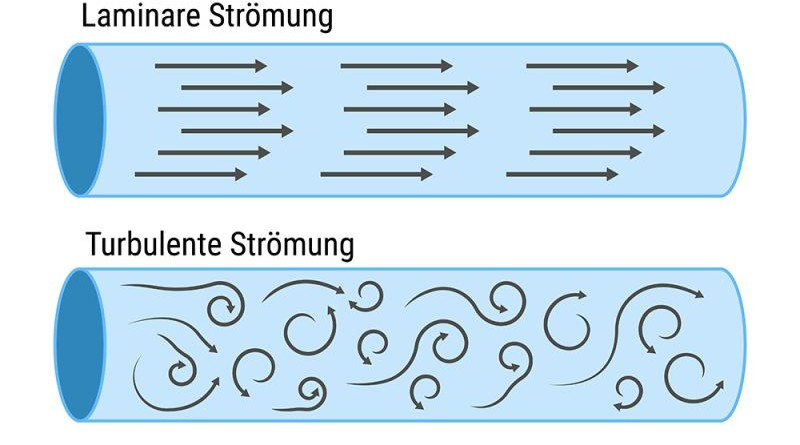
\includegraphics[width=\textwidth]{Bilder/stroeme.jpg}
        \caption{Laminare und turbulente Strömung. \cite{stroeme}}
        \label{fig:1}
    \end{minipage}
    \hfill
    \begin{minipage}{0.45\textwidth}
        \centering
        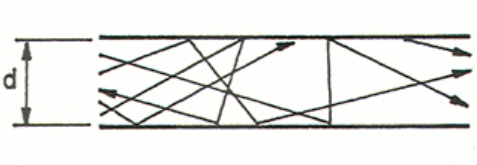
\includegraphics[width=\textwidth]{Bilder/molekular.png}
        \caption{Molekulare Strömung. \cite{molekular}}
        \label{fig:2}
    \end{minipage}
\end{figure}
\noindent In dem Experiment wird (für die Rechnungen) von einem idealen Gas 
ausgegangen. Das bedeutet, dass Moleküle als Punktmassen realisiert werden, 
das Eigenvolumen vernachlässigt wird und keine Wechselwirkungen bis auf elastische 
Stöße stattfinden. 

\subsection{Pumpen}
\subsubsection{Drehschieberpumpe}
\label{sec:dsp}
\begin{figure}[H]
    \centering
        \centering
        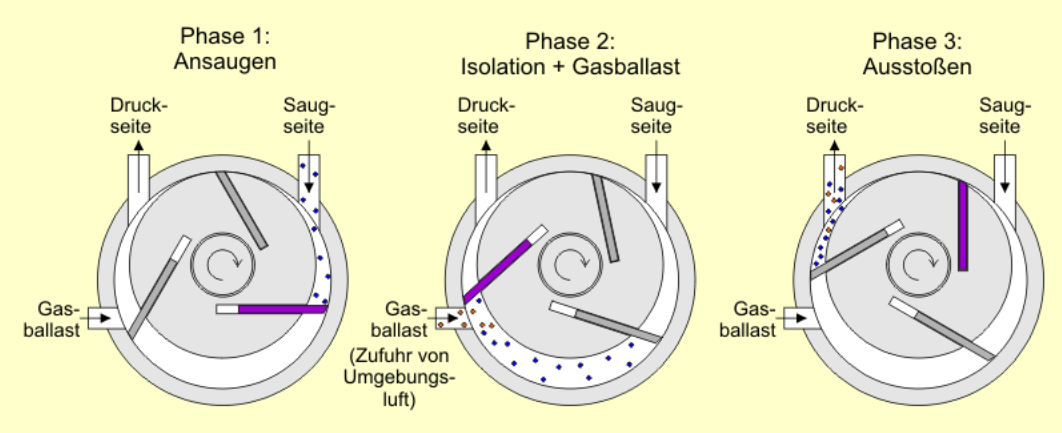
\includegraphics[width=0.9\textwidth]{Bilder/dsp.png}
        \caption{Schematischer Ablauf einer Drehschieberpumpe. \cite{glossar}}
    \hfill
    \label{fig:3}
\end{figure}

\subsubsection{Turbomolekularpumpe}
\label{sec:tmp}
\cite{glossar}